\documentclass{article}
\usepackage[utf8]{inputenc}

\title{Scientific Computing - Exercise Sheet 5}
\author{Jonathan Hellwig, Jule Schütt, Mika Tode, Giuliano Taccogna}
\date{\today}

\usepackage{float}
\usepackage{svg}
\usepackage{natbib}
\usepackage{graphicx}
\usepackage{caption}
\usepackage{algorithmicx}
\usepackage{algpseudocode}
\usepackage{enumitem}
\usepackage{amssymb}
\usepackage{amsmath}
\usepackage{color}

\begin{document}

\maketitle

\section{Exercise 1}
\begin{enumerate}[label=(\alph*)]
    \item Sketch of the mesh and the computational pattern:
	    \begin{align*}
        C=\left[\begin{matrix}
            1 & 17 & 33 & 49 & ...\\
            2 & 18 & 34 & 50 & ... \\
            3 & 19 & 35 & 51 & ... \\
            4 & \textbf{20} & 36 & 52 & ... \\
            \textbf{5} & |\overline{\underline{21}}| & \textbf{37} & 53 & ...\\
            6 & \textbf{22} & 38 & 54 & ... \\
            7 & 23 & 39 & 55 & ...\\
            8 & 24 & 40 & 56 & ... \\
            9 & 25 & 41 & 57 & ... \\
            10 & 26 & 42 & 58 & ... \\
	11 & 27 & 43 & 59  & ... \\
	12 & 28 & 44 & 60  & ... \\
	13 & 29 & 45 & 61  & ... \\
	14 & 30 & 46 & 62  & ... \\
	15 & 31 & 47 & 63  & ... \\
	16 & 32 & 48 & 64  & ... 
        \end{matrix}\right]
    \end{align*}
The computational pattern for grid point 21 is given by the fat numbers.    
    \item
    We will describe the average cache load for computing the next Laplace smoothing. The cache line length is 8 and we assume that if one data has been accessed, the following 7 entries were loaded instantly. That means if we load the third item, we loaded item 3 to item 10 in our cache. \\
    We will describe 3 different item positions
    \begin{itemize}
        \item Interior items:\\
    If we look on the sketch and choose one interior item $m$ of the mesh, we see that if we load the item above ($m-1$), then we always have load the item below ($m+1$), too. But the left item has the number $m-16$ and the right item has the number $m+16$. Thus, we have to load them separately. 
    \item Corner items:\\
    If we look on an corner item, we have one neighbour to the left or to the right and one neighbour above or below. with the same explanation as above it follows that we have to load two caches for the computation.
    
    \item Boundary items that were no corner items:\\
    If we look at an item on the side and not on the corner, there exists either 2 side neighbours (if we are at the top or at the bottom) and one neighbour above or below such that we have to load 3 caches.
    \\
    If the item is on the left or on the right side, there are two neighbours above and below and one neighbour either to the left or to the right. Then we have to load 2 caches.
    \end{itemize}
    There are 14 times 14 interior points, 4 corner points, 14 left side points as well as 14 right/bottom/top side point. All in all the average number of cache loads per computation is:
    \begin{align*}
        \frac{14\cdot14\cdot3+4\cdot2+14\cdot3+14\cdot3+14\cdot2+14\cdot2}{16\cdot16}=\frac{23}{8} = 2,875
    \end{align*}

    \item Sketch of the mesh which results from the Cuthill-McKee algorithm:
		    \begin{align*}
        C=\left[\begin{matrix}
          ... & ...  & ... & ... & ... &... & ... & ...\\
         27 & ...  & ... & ... & ... &... & ... & ...\\
	20 & 26 & ...  & ... & ... & ... &... & ...\\
	14 & 19 & 25 & ...  & ... & ... & ... & ...\\
	9 & 13 & 18 & 24  & ... & ... &... & ...\\
	5 & 8 & 12 & 17 & 23  & ... &... & ...\\
	2 & 4 & 7 & 11  & 16 & 22 & ... & ...\\
	0 & 1 & 3 & 6 & 10  & 15 & 21 & ... 
        \end{matrix}\right]
    \end{align*}
    
    \item 
 As one can see from the sketch if we look at interior item $x_{i,j}$, we need one cache line load to access te data value corrseponding to grid point $x_{i,j-1}$ (below),  this load gives the processor also access to the data value corresponding to grid point $x_{i-1,j}$ (on the left). The same holds for the grid points $x_{i+1,j}$ (on the right) and $x_{i,j+1}$ (above). That means 2 cache line loads are necessary for the 14 times 14 inner grid points.
\newline
For the 60 boundary and corner grid points at most 2 cache line loads are needed. But for example for the point 0 or 1 only one cache line load is necessary.
\newline
That means the average number of cache line loads is smaller than, but close to 2. 
\newpage

\end{enumerate}
\section{Exercise 2}
\begin{enumerate}[label=(\alph*)]

    \item The connectivity matrix $C\in\mathbb N^{10\times 10}$ of the mesh is the following:
    \begin{align*}
        C=\left[\begin{matrix}
            1 & 1 & 0 & 1 & 0 & 0 & 0 & 0 & 0 & 0\\
            1 & 1 & 1 & 0 & 0 & 0 & 0 & 0 & 0 & 1\\
            0 & 1 & 1 & 1 & 0 & 1 & 0 & 1 & 0 & 0\\
            1 & 0 & 1 & 1 & 1 & 0 & 0 & 0 & 0 & 0\\
            0 & 0 & 0 & 1 & 1 & 1 & 0 & 0 & 0 & 0\\
            0 & 0 & 1 & 0 & 1 & 1 & 1 & 0 & 0 & 0\\
            0 & 0 & 0 & 0 & 0 & 1 & 1 & 1 & 0 & 0\\
            0 & 0 & 1 & 0 & 0 & 0 & 1 & 1 & 1 & 0\\
            0 & 0 & 0 & 0 & 0 & 0 & 0 & 1 & 1 & 1\\
            0 & 1 & 0 & 0 & 0 & 0 & 0 & 0 & 1 & 1\\
        \end{matrix}\right]
    \end{align*}
    \item 
    
    \begin{figure}[h]
    \centering
     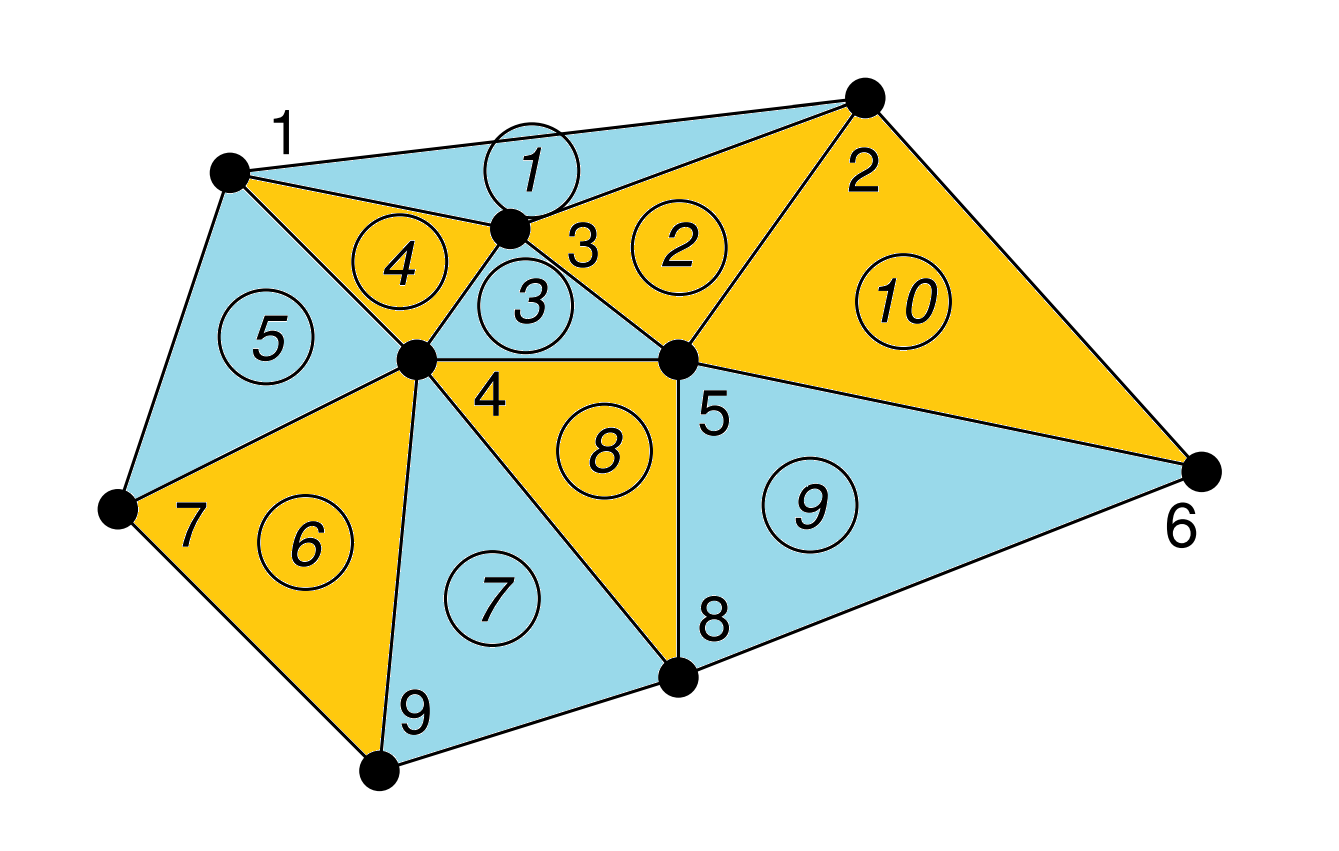
\includegraphics[scale=0.3]{erste Zerlegung}
    \caption{Inital Partition}
    \label{fig:meine-grafik}
    \end{figure}
Notation: i,j in the tables below, describes the edge, which seperates Element i and Element j. We write 1, if i is not in the same partition as j and 0 if i and j are in the same partition. c.w. stands for cut weight,  i.c. stands for interchange. That means in the i.c column, we state which elements are interchanged w.r.t the partition stated in the first row.
\newline
$\left(
 \begin{array}{cccccccccccc|c | c}
            1, 4 & 1, 2 & 4,5 & 3, 4 & 2, 3 & 2, 10 & 5, 6 & 3, 8 & 9,10 & 6, 7 & 7, 8 & 8,9 & \text{i.c} & \text{c.w}\\
	\hline
            1 & 1 & 1 & 1 & 1 & 0 & 1 & 1 & 1 & 1 & 1 & 1 & \text{Ini. Part.} & 11\\
	\hline
            1 & 0 & 0 & 0 & 1 & 0 & 1 & 1 & 1 & 1 & 1 & 1 &  1,4  & 8\\
	 0 & 1 & 1 & 1 & 0 & 1 & 1 & 1 & 1 & 1 & 1 & 1 &  1,2 & 10\\
 	0 & 1 & 1 & 0 & 1 & 0 & 0 & 1 & 1 & 1 & 1 & 1 &  4, 5 & 8\\
	\hline
	 0 & 1 & 0 & 1 & 0 & 0 & 1 & 0 & 1 & 1 & 1 & 1 &  3, 4 & \textbf{7}\\
	\hline
 	0 & 0 & 1 & 0 & 1 & 1 & 1 & 0 & 1 & 1 & 1 & 1 &  2, 3 & 8\\
	1 & 1 & 0 & 1 & 1 & 0 & 1 & 1 & 1 & 0 & 1 & 1 &  5, 6 & 9\\
	1 & 1 & 1 & 0 & 0 & 0 & 1 & 1 & 1 & 1 & 0 & 0 &  3, 8 & \textbf{7}\\
	1 & 1 & 1 & 1 & 1 & 1 & 1 & 1 & 1 & 1 & 1 & 0 &  9, 10 & 11\\
	1 & 1 & 1 & 1 & 1 & 0 & 0 & 1 & 1 & 1 & 0 & 1 &  6, 7 & 9\\
	1 & 1 & 1 & 1 & 1 & 0 & 1 & 0 & 1 & 0 & 1 & 0 &  7,8 & 8\\
	1 & 1 & 1 & 1 & 1 & 0 & 1 & 0 & 0 & 1 & 0 & 1 & 8, 9 & 8\\
   \end{array}
\right)$
\newline
Interchange Element 3 and 4:

    \begin{figure}[h]
    \centering
     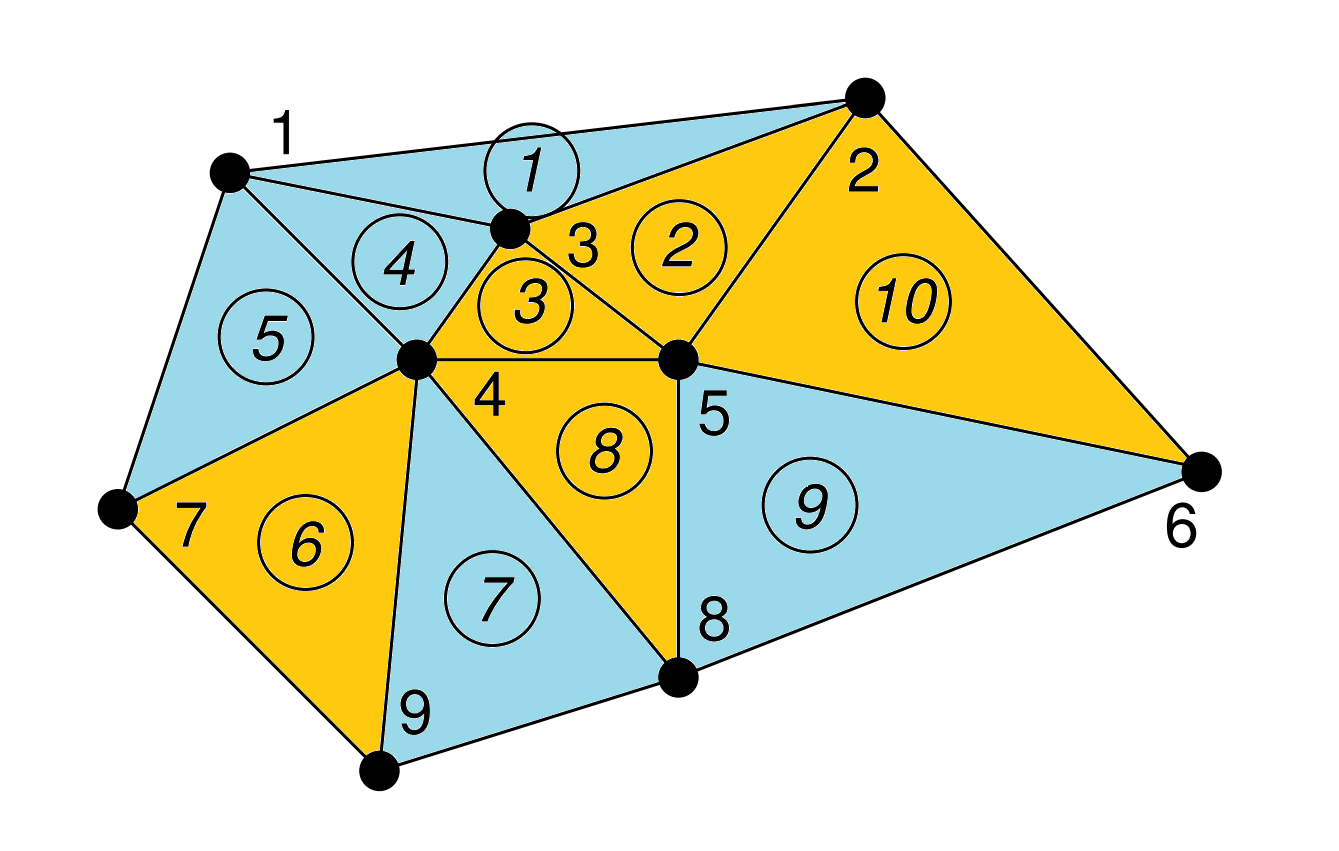
\includegraphics[scale=0.3]{zweite Zerlegung}
    \caption{Second Partition}
    \label{fig:meine-grafik2}
    \end{figure}

$\left(
 \begin{array}{cccccccccccc|c | c}
            1, 4 & 1, 2 & 4,5 & 3, 4 & 2, 3 & 2, 10 & 5, 6 & 3, 8 & 9,10 & 6, 7 & 7, 8 & 8,9 & \text{i.c} & \text{c.w}\\
	\hline
            0 & 1 & 0 & 1 & 0 & 0 & 1 & 0 & 1 & 1 & 1 & 1 &  \text{2. Part.} & 7\\
	\hline
            1 & 1 & 0 & 1 & 1 & 1 & 1 & 0 & 1 & 1 & 1 & 1 &  1,2  & 10\\
	 1 & 1 & 1 & 1 & 1 & 0 & 1 & 1 & 1 & 1 & 1 & 1 &  3,4 & 11\\
 	0 & 1 & 1 & 1 & 0 & 0 & 1 & 0 & 1 & 0 & 1 & 1 &  5, 6 & 7\\
	 0 & 1 & 0 & 1 & 0 & 0 & 0 & 0 & 1 & 1 & 0 & 1 &  9,10 & 7\\
	\hline
 	0 & 1 & 0 & 1 & 0 & 0 & 0 & 0 & 1 & 1 & 0 & 1 &  6,7 & \textbf{5}\\
	\hline
	0 & 1 & 0 & 1 & 0 & 0 & 1 & 1 & 1 & 0 & 1 & 0 &  7,8 & 6\\
	0 & 1 & 0 & 1 & 0 & 0 & 1 & 1 & 1 & 0 & 1 & 0 &  8, 9 & 6
   \end{array}
\right)$
\newline
 Interchange element 6 and 7:
    \begin{figure}[h]
    \centering
     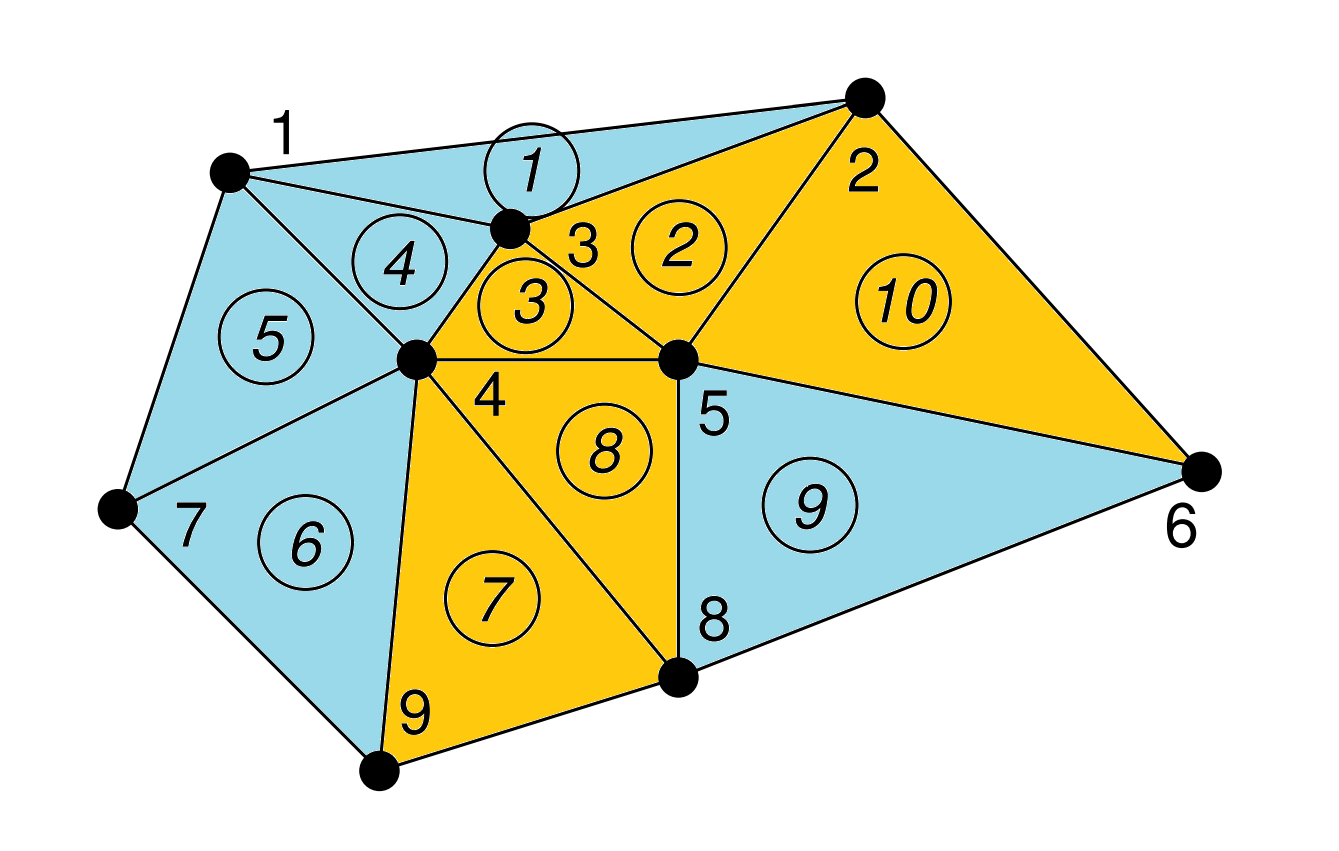
\includegraphics[scale=0.3]{dritte Zerlegung}
    \caption{3. Partition}
    \label{fig:meine-grafik3}
    \end{figure}
    
$\left(
 \begin{array}{cccccccccccc|c | c}
            1, 4 & 1, 2 & 4,5 & 3, 4 & 2, 3 & 2, 10 & 5, 6 & 3, 8 & 9,10 & 6, 7 & 7, 8 & 8,9 & \text{i.c} & \text{c.w}\\
	\hline
            0 & 0 & 1 & 0 & 1 & 1 & 1 & 0 & 1 & 1 & 1 & 1 &  \text{3. Part.} & \textbf{5}\\
	\hline
            1 & 1 & 0 & 1 & 1 & 1 & 1 & 0 & 1 & 0 & 1 & 0 &  1,2  & 8\\
	 1 & 1 & 1 & 1 & 1 & 0 & 1 & 1 & 1 & 0 & 1 & 0 &  3,4 & 9\\
 	0 & 1 & 0 & 1 & 0 & 1 & 0 & 0 & 1 & 1 & 0 & 0 &  9,10 & \textbf{5}\\
	 0 & 1 & 0 & 1 & 0 & 0 & 1 & 0 & 1 & 1 & 0 & 1 &  6, 7& 6\\
 	0 & 1 & 0 & 1 & 0 & 0 & 0 & 1 & 0 & 1 & 1 & 1 &  8, 9 & 6

   \end{array}
\right)$
\newline
No further improvement, the algorithm terminates.
\end{enumerate}
\end{document}